\documentclass[aspectratio=169,10pt]{beamer}

\usetheme{Madrid}
\usecolortheme{seahorse}
\usefonttheme{professionalfonts}
\setbeamertemplate{footline}[frame number]
\setbeamertemplate{navigation symbols}{}

%--------------------------------------------------------------
% Packages
%--------------------------------------------------------------
\usepackage{amsmath,amssymb,amsfonts}
\usepackage{mathtools}
\usepackage{bm}
\usepackage{booktabs}
\usepackage{graphicx}
\usepackage{listings}
\usepackage{xcolor}
\usepackage{tikz}
\usepackage{array}
\usepackage{multicol}

\graphicspath{{figures/}}

%--------------------------------------------------------------
% Listings: Python style
%--------------------------------------------------------------
\lstdefinestyle{python}{
  language=Python,
  basicstyle=\ttfamily\scriptsize,
  numbers=left,
  numberstyle=\tiny\color{gray},
  frame=single,
  backgroundcolor=\color{gray!7},
  keywordstyle=\color{blue}\bfseries,
  commentstyle=\color{green!50!black}\itshape,
  stringstyle=\color{red!70!black},
  breaklines=true,
  tabsize=4,
  showstringspaces=false,
  captionpos=b,
}
\lstset{style=python}

%--------------------------------------------------------------
% Convenience macros
%--------------------------------------------------------------
\newcommand{\mHH}{\mathcal H}
\newcommand{\inner}[2]{\langle #1, #2 \rangle}
\newcommand{\norm}[1]{\left\|#1\right\|}
\newcommand{\Fix}{\mathrm{Fix}}
\newcommand{\R}{\mathbb{R}}
\newcommand{\Id}{\mathrm{Id}}

%--------------------------------------------------------------
% Title
%--------------------------------------------------------------
\title[KM Method -- Ch.5]{The Krasnosel'ski\u{i}-Mann Iterative Method}
\subtitle{Chapter 5: The Inertial Krasnosel'ski\u{i}-Mann Iteration}
\author{Based on Dong, Cho, He, Pardalos \& Rassias}
\date{\today}

\begin{document}

%--------------------------------------------------------------
\begin{frame}
  \titlepage
\end{frame}

%--------------------------------------------------------------
\begin{frame}{Table of Contents}
  \tableofcontents
\end{frame}

%==============================================================
\section{Notation Recap and What ``Inertia'' Means}
%==============================================================

\begin{frame}[allowframebreaks]{Notation You'll Need / Recap}

  \textbf{Where we left off (Chapter 3).}  For a nonexpansive
  operator $T:\mHH\to\mHH$ (meaning $\norm{Tx-Ty}\le\norm{x-y}$
  for all $x,y$) with $\Fix(T)=\{x\in\mHH : Tx=x\}\neq\emptyset$,
  the \textbf{Krasnosel'ski\u{i}-Mann (KM) iteration} is
  \[
    x_{n+1} = (1-\lambda_n)x_n + \lambda_n T(x_n), \qquad n\ge 0,
  \]
  where $\lambda_n\in(0,1)$ is the \textbf{relaxation parameter}.
  Under mild conditions on $\{\lambda_n\}$ (e.g.\ $\inf_n\lambda_n>0$,
  $\sup_n\lambda_n<1$), $x_n$ converges weakly to a point of
  $\Fix(T)$.  This chapter asks: \emph{can we reach that fixed
  point in fewer iterations, without changing $T$ or the cost per
  step?}

  \vspace{0.5em}
  \textbf{Plain-English idea: add momentum.}  Instead of moving
  from $x_n$ purely toward $T(x_n)$, we first give the iterate a
  ``nudge'' in the direction it was \emph{already} moving, and only
  then apply the KM update.  This nudge is called the
  \textbf{inertial term}.

  \begin{block}{The Inertial Term $\theta_n(x_n - x_{n-1})$}
    \[
      \theta_n\,(x_n - x_{n-1})
    \]
    \begin{itemize}
      \item $x_n - x_{n-1}$ is the \emph{last move} the algorithm
            made --- literally the previous step's displacement
            vector.
      \item $\theta_n\in[0,1)$ (theta sub $n$) is the
            \textbf{inertial parameter}: how large a fraction of
            the last move to repeat.
      \item Plain English: ``add a fraction of your last move
            again, like momentum'' --- if you were moving fast in
            some direction, keep some of that speed instead of
            starting from rest at every step.
    \end{itemize}
  \end{block}

  \framebreak

  \begin{block}{The Auxiliary Point $y_n$}
    \[
      y_n = x_n + \theta_n(x_n - x_{n-1})
    \]
    $y_n$ (read ``$y$ sub $n$'') is \emph{not} a new iterate kept
    around forever --- it is a temporary, extrapolated point
    computed \emph{before} applying $T$.  The KM-type update is
    then applied at $y_n$ instead of at $x_n$:
    \[
      x_{n+1} = (1-\lambda_n)y_n + \lambda_n T(y_n).
    \]
    Intuitively: $y_n$ is ``where momentum carries you to'' before
    you look at the operator $T$ again.
  \end{block}

  \textbf{What do ``alternated'' and ``online'' mean?}
  \begin{itemize}
    \item \textbf{Alternated inertial}: apply the inertial nudge
          only on \emph{every other} iteration (e.g.\ odd $n$), and
          use $y_n = x_n$ (no nudge) on the remaining iterations.
          Plain English: ``momentum, then a plain KM step to
          re-stabilize, then momentum again, \ldots'' This periodic
          ``resetting'' restores a monotonically decreasing error,
          which pure inertial methods can lose.
    \item \textbf{Online inertial}: instead of prescribing
          $\theta_n$ by a fixed formula in advance, \emph{adapt}
          $\theta_n$ on the fly using quantities you can actually
          observe during the run (ratios of consecutive step
          sizes), together with an automatic \emph{restart} rule
          that falls back to $\theta_n=0$ whenever the observed
          progress is not good enough to guarantee convergence.
          Plain English: ``let the algorithm tune its own
          momentum based on how well it is currently doing.''
  \end{itemize}

\end{frame}

%==============================================================
\section{5.1 General Inertial Krasnosel'ski\u{i}-Mann Iterations}
%==============================================================

\begin{frame}[allowframebreaks]{5.1 Motivation: From the Heavy Ball to Inertial KM}

  \textbf{Physical intuition first.}  Imagine a heavy ball rolling
  down a bumpy hill toward a target at the bottom.  A ``memoryless''
  particle that always moves in the direction of steepest descent
  can get stuck oscillating in a small dip or bump.  A \emph{heavy}
  ball, however, carries momentum: it keeps rolling in roughly the
  direction it was already going, so it can \emph{coast through}
  small bumps and reach the target faster.  Formally this is
  Polyak's 1964 \textbf{heavy ball with friction} dynamical system.

  \begin{center}
    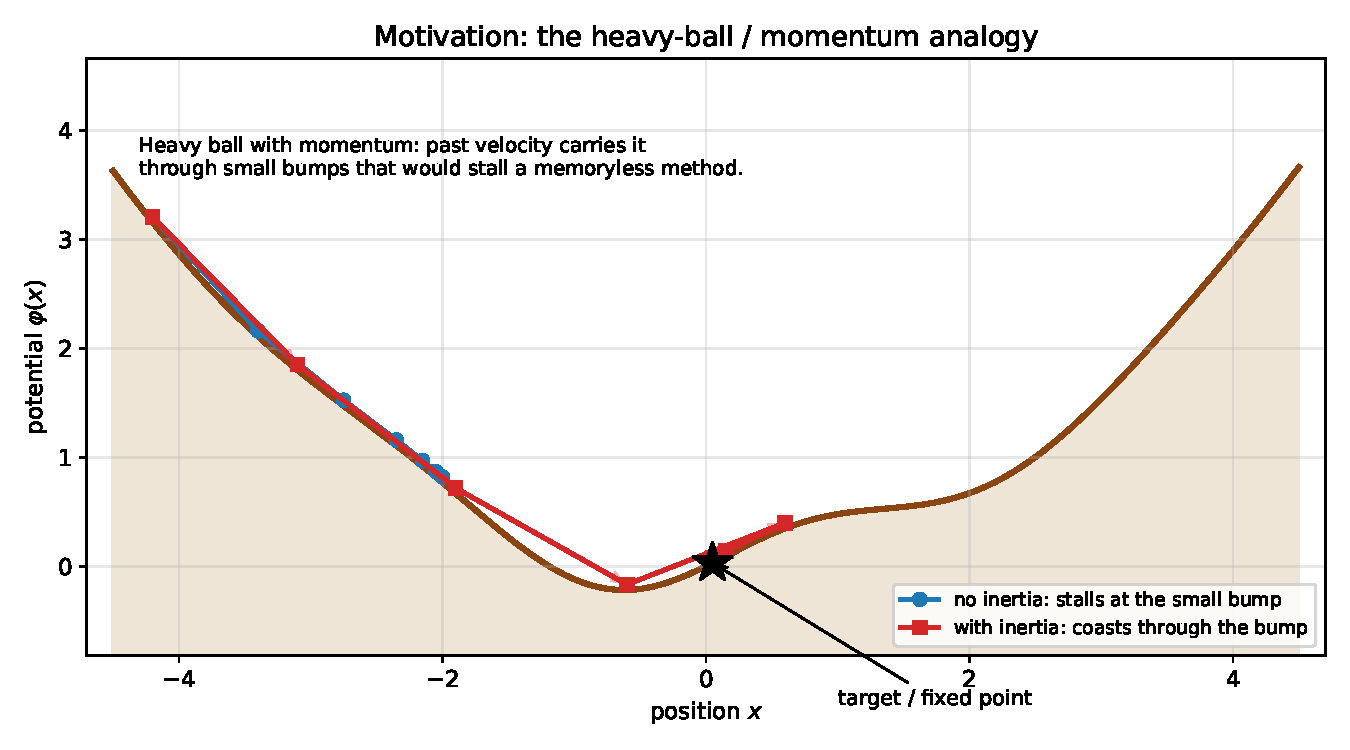
\includegraphics[width=0.75\textwidth]{heavy_ball_schematic}
  \end{center}

  \framebreak

  \begin{block}{Heavy Ball with Friction ODE}
    \[
      \ddot x(t) + \gamma(t)\dot x(t) + \nabla\varphi(x(t)) = 0
    \]
    \begin{itemize}
      \item $x(t)$ is the position of the ``ball'' at time $t$;
            $\dot x(t)$ its velocity; $\ddot x(t)$ its acceleration
            (Newton's second law, unit mass).
      \item $\gamma(t)>0$ is a \textbf{friction} coefficient: it
            damps the velocity so the ball eventually settles.
      \item $\varphi$ is a differentiable potential function (the
            ``hill''); $-\nabla\varphi(x(t))$ is the ``gravity''
            force pulling the ball downhill.
      \item Reading the equation: mass$\times$acceleration $+$
            friction$\times$velocity $+$ gravity force $= 0$.
    \end{itemize}
  \end{block}

  \textbf{Why this matters for KM iterations:} discretizing this
  ODE in time produces exactly the inertial-term structure
  $\theta_n(x_n-x_{n-1})$ we saw on the previous slide.  We now
  derive that connection step by step.

\end{frame}

\begin{frame}[allowframebreaks]{5.1 Derivation: ODE $\to$ Discretization $\to$ Inertial Update}

  \textbf{Step 1 --- discretize time.}  Replace the continuous
  time derivative by finite differences with step size $h_n>0$ at
  time $t_n$, writing $x_n\approx x(t_n)$:
  \[
    \dot x(t_n)\approx\frac{x_n - x_{n-1}}{h_n},
    \qquad
    \ddot x(t_n)\approx\frac{x_{n+1}-2x_n+x_{n-1}}{h_n^2}.
  \]

  \textbf{Step 2 --- plug into the ODE.}  With
  $\gamma_n=\gamma(t_n)$, the heavy ball ODE becomes the
  \emph{explicit finite-difference discretization}:
  \begin{block}{Explicit Discretization of the Heavy Ball ODE}
    \[
      \frac{x_{n+1}-2x_n+x_{n-1}}{h_n^2}
      + \gamma_n\frac{x_n-x_{n-1}}{h_n}
      + \nabla\varphi(x_n) = 0, \qquad n\ge 1.
    \]
  \end{block}

  \textbf{Step 3 --- solve for $x_{n+1}$.}  Multiply through by
  $h_n^2$ and isolate $x_{n+1}$:
  \[
    x_{n+1} = x_n + \underbrace{(1-\gamma_n h_n)}_{=:\mu_n}(x_n-x_{n-1})
    - \underbrace{h_n^2}_{=:\nu_n}\nabla\varphi(x_n),
    \quad n\ge 1.
  \]

  \framebreak

  \textbf{Step 4 --- name the pieces.}  Setting
  $\mu_n = 1-\gamma_n h_n$ (the \emph{inertial parameter}) and
  $\nu_n=h_n^2$ (the \emph{step size}), the update splits into two
  readable lines --- exactly the extrapolate-then-move pattern:
  \begin{block}{Polyak's Inertial Extrapolation Algorithm}
    \[
      \begin{cases}
        z_n = x_n + \mu_n(x_n - x_{n-1}), \\
        x_{n+1} = z_n - \nu_n\nabla\varphi(x_n),
      \end{cases}
      \qquad n\ge 1.
    \]
    $z_n$ is the extrapolated (momentum-carried) point; $\mu_n$
    controls how much inertia is kept; $\nu_n$ is the gradient
    step size at the \emph{current} point $x_n$ (not $z_n$).
    Polyak called $\mu_n(x_n-x_{n-1})$ the \textbf{inertial term}
    and $\{\mu_n\}$ the \textbf{inertial parameter sequence}.
  \end{block}

  \textbf{Step 5 --- Nesterov's variant.}  Nesterov's accelerated
  gradient method uses the \emph{same} extrapolated point $z_n$
  \emph{inside} the gradient too:
  \begin{block}{Nesterov's Accelerated Gradient (contrast)}
    \[
      \begin{cases}
        z_n = x_n + \mu_n(x_n-x_{n-1}), \\
        x_{n+1} = z_n - \nu_n\nabla\varphi(z_n).
      \end{cases}
    \]
    The only difference from Polyak's scheme is
    $\nabla\varphi(x_n)\to\nabla\varphi(z_n)$: the gradient is
    evaluated at the \emph{extrapolated} point, not the current
    one. Careful choice of $\{\mu_n\}$ is known to accelerate the
    theoretical functional convergence rate from $O(1/n)$ to
    $O(1/n^2)$ or $o(1/n^2)$.
  \end{block}

  \framebreak

  \textbf{Step 6 --- replace ``move downhill'' by ``apply $T$''.}
  In fixed-point theory there is no potential $\varphi$; instead we
  have a nonexpansive operator $T$.  Mainge's key idea: swap the
  gradient step for a KM-type averaging step against $T$.  This is
  the same discretization idea as Steps 1--4, but now applied to
  fixed-point iterations rather than smooth optimization.

  \begin{block}{Classical Inertial Krasnosel'ski\u{i}-Mann Iteration}
    For each $n\ge 1$:
    \[
      \begin{cases}
        y_n = x_n + \alpha_n(x_n - x_{n-1}), \\
        x_{n+1} = (1-\lambda_n)y_n + \lambda_n T(y_n),
      \end{cases}
    \]
    where $\alpha_n$ plays the role of $\mu_n$ (inertial parameter)
    and $\lambda_n\in(0,1)$ is the usual KM relaxation parameter.
    $T$ is applied at the \emph{extrapolated} point $y_n$, mirroring
    Nesterov's choice above.
  \end{block}

  \begin{alertblock}{Convergence Conditions (Mainge)}
    The sequence $\{x_n\}$ converges weakly to a point of
    $\Fix(T)$ provided:
    \begin{itemize}
      \item[(C1)] $\{\alpha_n\}\subseteq[0,\alpha]$ for some
            $\alpha\in[0,1)$;
      \item[(C2)] $\sum_{n=0}^{\infty}\alpha_n\norm{x_n-x_{n-1}}^2
            <+\infty$ (a \emph{summable} condition --- it involves
            the iterates themselves, so $\alpha_n$ must often be
            computed on the fly);
      \item[(C3)] $\inf_{n\ge0}\lambda_n>0$ and
            $\sup_{n\ge0}\lambda_n<1$.
    \end{itemize}
  \end{alertblock}

\end{frame}

\begin{frame}[allowframebreaks]{5.1 Simplifying the Conditions: Bo\c{t}--Csetnek and Beyond}

  \textbf{Why simplify?}  Condition (C2) above is awkward: it is a
  summability condition on a quantity that depends on the (not yet
  known) iterates $x_n$.  Bo\c{t} and Csetnek removed (C2) entirely
  and replaced (C1), (C3) by conditions that can be checked
  \emph{in advance}.

  \begin{block}{Bo\c{t}--Csetnek Conditions (D1)--(D2)}
    \begin{itemize}
      \item[(D1)] $\{\alpha_n\}\subseteq[0,\alpha]$ is
            \textbf{nondecreasing} with $\alpha_1=0$ and
            $0\le\alpha<1$;
      \item[(D2)] For each $n\ge1$, with $\lambda,\sigma,\delta>0$:
      \[
        \delta > \frac{\alpha^2(1+\alpha)+\alpha\sigma}{1-\alpha^2},
        \qquad
        0<\lambda\le\lambda_n\le
        \frac{\delta-\alpha[\alpha(1+\alpha)+\alpha\delta+\sigma]}
             {\delta[1+\alpha(1+\alpha)+\alpha\delta+\sigma]}.
      \]
    \end{itemize}
  \end{block}

  Here $\alpha$ (the cap on the inertial parameter), $\sigma$, and
  $\delta$ are free positive constants that the user chooses to
  fit a valid range of relaxation parameters $\lambda_n$; larger
  $\alpha$ (more inertia) forces a \emph{smaller} admissible range
  for $\lambda_n$.  This trade-off between ``how much inertia'' and
  ``how large a relaxation parameter is still safe'' recurs
  throughout the chapter.

  \framebreak

  \textbf{Beyond nonnegative inertia.}  All the conditions above
  assume $\alpha_n,\beta_n\ge0$.  Dong et al.\ showed convergence
  still holds if one of the two inertial parameters is allowed to
  be \emph{negative} (i.e.\ the extrapolation can point
  \emph{backward}), covering two additional regimes:
  \begin{itemize}
    \item Case 1: $\alpha_n\in[0,1]$, $\beta_n\in(-\infty,0]$;
    \item Case 2: $\alpha_n\in[-1,0]$, $\beta_n\in[0,+\infty)$.
  \end{itemize}
  This considerably broadens the family of provably convergent
  inertial KM schemes beyond the ``both parameters nonnegative''
  picture.

\end{frame}

\begin{frame}[allowframebreaks]{5.1 The General Inertial KM Iteration}

  \textbf{Two extrapolation points instead of one.}  Dong et al.\
  observed that using the \emph{same} extrapolated point both as
  the ``momentum carrier'' $y_n$ and as the argument of $T$ is a
  special case of something more flexible: let the momentum
  applied \emph{before} averaging differ from the momentum applied
  \emph{inside} $T$.

  \begin{block}{General Inertial Krasnosel'ski\u{i}-Mann Iteration}
    For each $n\ge1$:
    \[
      \begin{cases}
        y_n = x_n + \alpha_n(x_n-x_{n-1}), \\
        z_n = x_n + \beta_n(x_n-x_{n-1}), \\
        x_{n+1} = (1-\lambda_n)y_n + \lambda_n T(z_n),
      \end{cases}
    \]
    where $\{\alpha_n\},\{\beta_n\},\{\lambda_n\}\subseteq[0,1]$.
    $y_n$ is the extrapolated point used in the \emph{averaging}
    (outside $T$); $z_n$ is the (possibly different) extrapolated
    point fed \emph{into} $T$.
  \end{block}

  \textbf{Why generalize?}  Because this single scheme
  \emph{contains} several previously separate methods as special
  cases --- so one convergence theorem covers them all.

  \framebreak

  \begin{block}{Special Cases (Remark 5.2)}
    \begin{itemize}
      \item $\alpha_n=\beta_n$ (so $y_n=z_n$): recovers the
            \textbf{classical inertial KM iteration} above.
      \item $\beta_n=0$ (no momentum fed into $T$): the
            \textbf{accelerated KM iteration}
            \[
              y_n = x_n+\alpha_n(x_n-x_{n-1}),\quad
              x_{n+1}=\lambda_n y_n+(1-\lambda_n)T(x_n),
            \]
            which is exactly the explicit discretization of
            $\ddot x(t)+\gamma(t)\dot x(t)+(\Id-T)(x(t))=0$ ---
            the heavy ball ODE with $\nabla\varphi$ replaced by
            the ``fixed-point residual'' $\Id-T$.
      \item $\alpha_n=0$ (no momentum outside $T$): the
            \textbf{reflected KM iteration}
            \[
              z_n = x_n+\beta_n(x_n-x_{n-1}),\quad
              x_{n+1}=(1-\lambda_n)x_n+\lambda_n T(z_n).
            \]
    \end{itemize}
  \end{block}

  \begin{alertblock}{Theorem 5.1 (Dong et al.)}
    Let $T:\mHH\to\mHH$ be nonexpansive with $\Fix(T)\neq\emptyset$.
    If $\{\alpha_n\}\subset[0,\alpha]$, $\{\beta_n\}\subset[0,\beta]$
    are nondecreasing with $\alpha_1=\beta_1=0$,
    $\alpha,\beta\in[0,1)$, $\lambda_n\equiv\lambda$, and a
    Bo\c{t}--Csetnek-style bound on $\lambda$ (using
    $\xi=\max\{\alpha,\beta\}$ in place of $\alpha$) holds, then
    $\{x_n\}$ converges weakly to a point of $\Fix(T)$.
  \end{alertblock}

\end{frame}

\begin{frame}{5.1 Worked Example --- Setting Up the Running Problem}

  \textbf{Running example (unit-disk projection).}  Let
  $\mHH=\R^2$, $C=\{x:\norm{x}\le1\}$ the closed unit disk, and let
  $T=P_C$ be the (nonexpansive, in fact firmly nonexpansive)
  metric projection onto $C$:
  \[
    T(x)=P_C(x)=
    \begin{cases}
      x, & \norm{x}\le1,\\
      x/\norm{x}, & \norm{x}>1.
    \end{cases}
  \]
  We take $x_0=(3,4)$, so $\norm{x_0}=5$.  The unique fixed point
  reached from this starting ray is $x^*=x_0/\norm{x_0}=(0.6,0.8)$.

  \begin{alertblock}{Key structural fact used throughout}
    Write $u=(0.6,0.8)$ (unit vector).  If $x_{-1}=x_0=5u$ (i.e.\
    we start with \emph{zero} initial velocity, a common
    convention), then \emph{every} iterate of both plain KM and
    inertial KM stays on the ray $\{ru : r\in\R\}$: we may track
    the single scalar $r_n$ with $x_n=r_nu$ instead of a full 2-D
    vector. This lets us compare convergence speeds with concrete
    numbers.
  \end{alertblock}

  For $r>0$: $T(ru)=u$ if $r>1$, and $T(ru)=ru$ if $r\le1$ ---
  applying $T$ simply clips the scalar $r$ down to $1$ once
  $r\le 1$ it leaves $r$ unchanged (already feasible).

\end{frame}

\begin{frame}[allowframebreaks]{5.1 Worked Example --- Inertial KM by Hand}

  \textbf{Setup.}  $\lambda_n\equiv\lambda=0.5$ (constant
  relaxation), $\theta_n\equiv\theta=0.2$ (constant inertial
  parameter), $x_{-1}=x_0$, $r_0=5$.  Along the ray, the update
  becomes purely scalar:
  \[
    s_n = r_n + \theta(r_n-r_{n-1}), \qquad
    r_{n+1} =
    \begin{cases}
      (1-\lambda)s_n+\lambda, & s_n>1,\\
      s_n, & s_n\le1.
    \end{cases}
  \]

  \textbf{Step-by-step (first few iterations):}
  \begin{itemize}
    \item $n=0$: $s_0 = 5+0.2(5-5)=5.0$ (no inertial effect yet,
          since $r_{-1}=r_0$); $r_1=0.5(5.0)+0.5=3.0$.
    \item $n=1$: $s_1=3.0+0.2(3.0-5.0)=2.6$; $r_2=0.5(2.6)+0.5=1.8$.
    \item $n=2$: $s_2=1.8+0.2(1.8-3.0)=1.56$; $r_3=0.5(1.56)+0.5=1.28$.
    \item $n=3$: $s_3=1.28+0.2(1.28-1.8)=1.176$; $r_4=0.5(1.176)+0.5=1.088$.
    \item $n=4$: $s_4=1.088+0.2(1.088-1.28)=1.0496$; $r_5=1.0248$.
    \item $n=5$: $s_5=1.0248+0.2(1.0248-1.088)=1.01216$; $r_6=1.00608$.
    \item $n=6$: $s_6=1.00608+0.2(1.00608-1.0248)=1.002336$; $r_7=1.001168$.
    \item $n=7$: $s_7=1.001168+0.2(1.001168-1.00608)=1.0001856$;
          $r_8=1.0000928$.
  \end{itemize}

  \framebreak

  \begin{block}{Comparison Table: $|r_n-1|$ (distance to $r^*=1$)}
    \centering\footnotesize
    \begin{tabular}{c|ccccccccccccc}
      \toprule
      $n$ & 0 & 1 & 2 & 3 & 4 & 5 & 6 & 7 & 8 & 9 & 10 & 11 & 12\\
      \midrule
      Plain KM & 4 & 2 & 1 & 0.5 & 0.25 & 0.125 & 0.0625 & 0.0313 &
        0.0156 & 0.0078 & 0.0039 & 0.0020 & \textbf{0.00098}\\
      Inertial KM & 4 & 2 & 0.8 & 0.28 & 0.088 & 0.0248 & 0.0061 &
        0.0012 & \textbf{0.000093} & --- & --- & --- & ---\\
      \bottomrule
    \end{tabular}
  \end{block}

  \begin{alertblock}{Concrete speed-up}
    To reach tolerance $|r_n-1|<10^{-3}$:
    \begin{itemize}
      \item \textbf{Plain KM} (recursion $r_{n+1}-1=0.5(r_n-1)$,
            i.e.\ $|r_n-1|=4\cdot0.5^n$) needs
            $\boxed{n=12}$ iterations ($|r_{12}-1|\approx 0.000977$).
      \item \textbf{Inertial KM} ($\theta=0.2$) needs only
            $\boxed{n=8}$ iterations
            ($|r_8-1|\approx 0.0000928$) --- \textbf{33\% fewer
            iterations} for the same tolerance, at essentially the
            same cost per step (one extra vector subtraction and
            scalar multiply per iteration).
    \end{itemize}
  \end{alertblock}

\end{frame}

\begin{frame}{5.1 Worked Example --- Figures}

  \begin{center}
    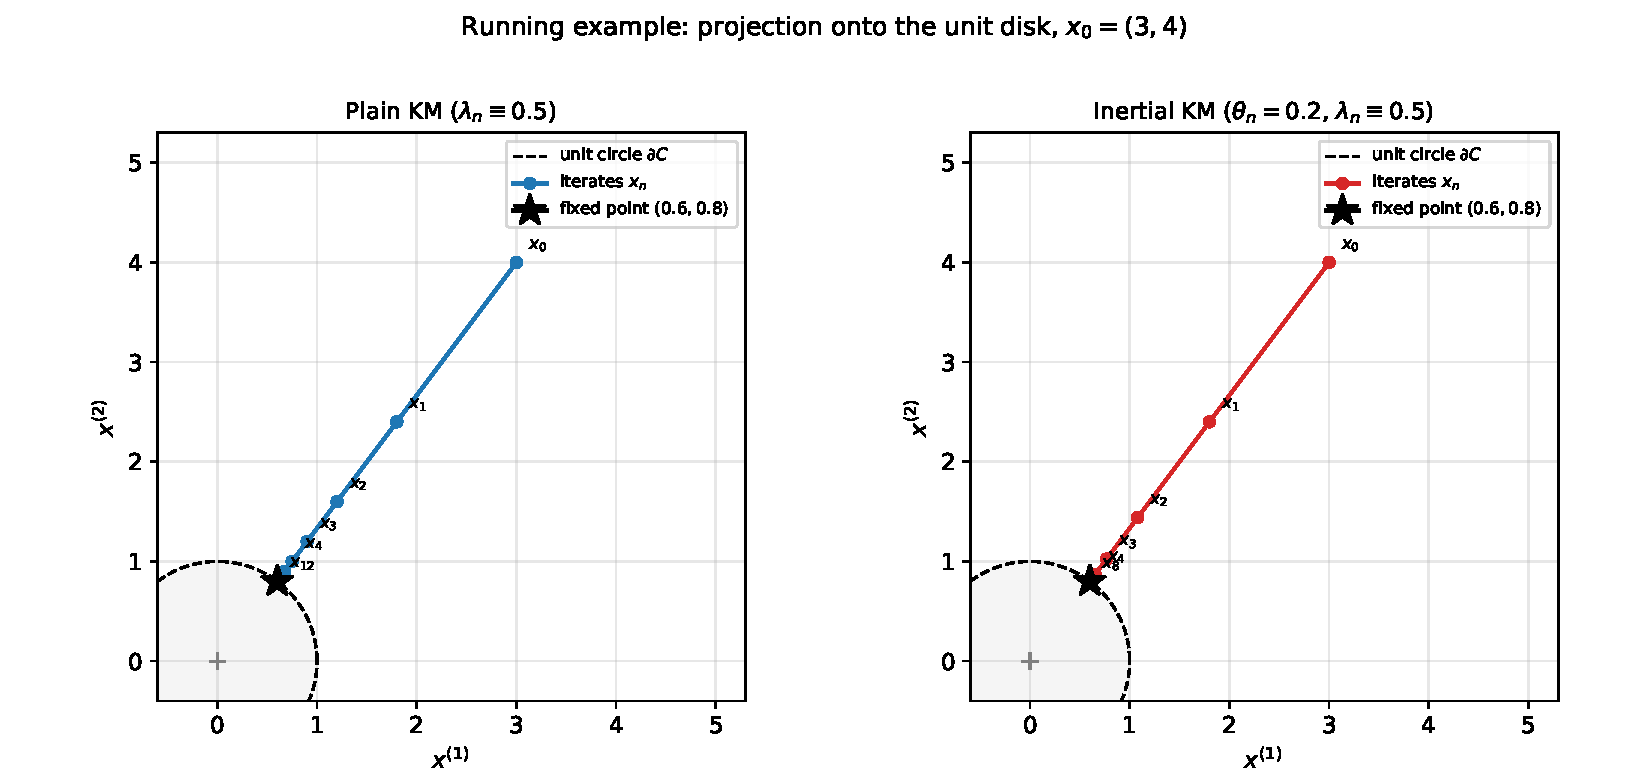
\includegraphics[width=0.92\textwidth]{km_vs_inertial_km}
  \end{center}
  \footnotesize Both methods stay on the ray through $(0.6,0.8)$;
  inertial KM (right) reaches the boundary of the disk in
  noticeably fewer, larger steps than plain KM (left).

\end{frame}

\begin{frame}{5.1 Worked Example --- Convergence Curves}

  \begin{center}
    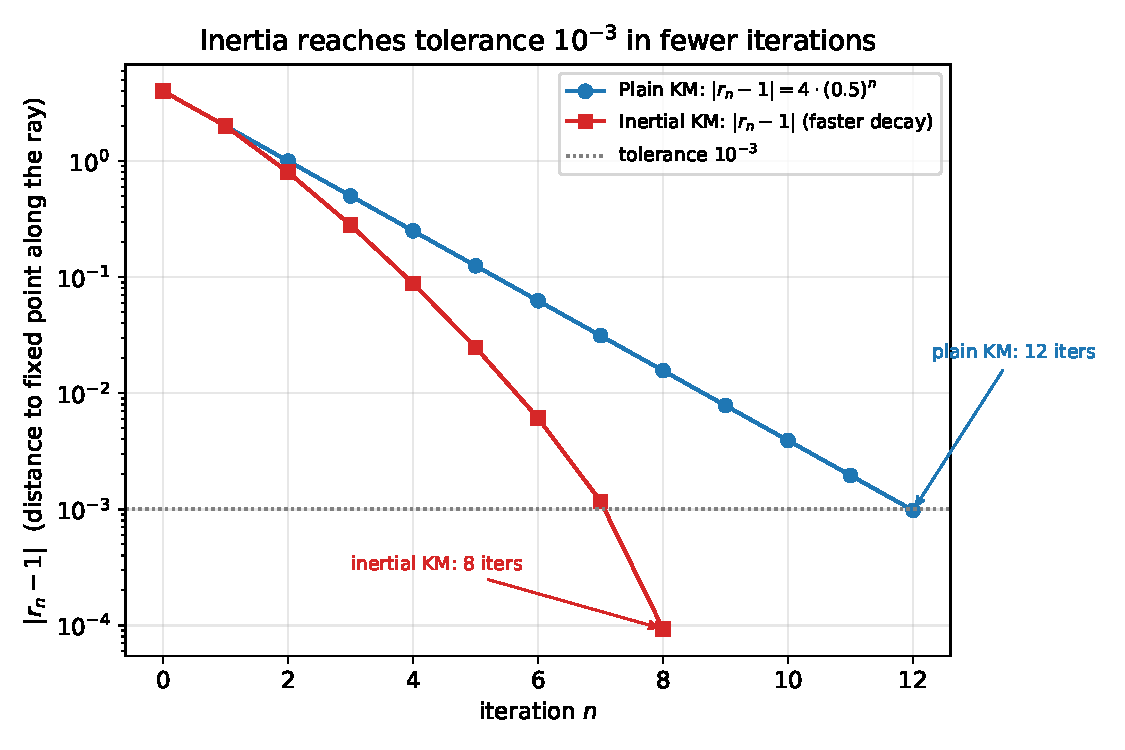
\includegraphics[width=0.78\textwidth]{rn_convergence}
  \end{center}
  \footnotesize Semilog plot of $|r_n-1|$: the inertial curve
  (red) drops below the $10^{-3}$ tolerance line after only 8
  iterations, versus 12 for plain KM (blue). Both decay
  geometrically, but the inertial scheme has a much smaller
  effective contraction factor at each step.

\end{frame}

\begin{frame}[fragile]{5.1 Python: General Inertial KM Iteration}
\begin{lstlisting}[caption={General inertial KM iteration (Python/NumPy)}]
import numpy as np

def project_unit_disk(x):
    """T = projection onto the closed unit disk (nonexpansive)."""
    n = np.linalg.norm(x)
    return x if n <= 1.0 else x / n

def general_inertial_km(T, x0, alpha_seq, beta_seq, lam_seq, n_iter):
    """
    yn = xn + alpha_n (xn - x_{n-1})   -- extrapolation OUTSIDE T
    zn = xn + beta_n  (xn - x_{n-1})   -- extrapolation INSIDE T
    x_{n+1} = (1-lam_n) yn + lam_n T(zn)
    Special cases: alpha_n=beta_n -> classical inertial KM;
                   beta_n=0       -> accelerated KM;
                   alpha_n=0      -> reflected KM.
    """
    xprev = x0.copy()
    x = x0.copy()
    hist = [x.copy()]
    for n in range(n_iter):
        a, b, lam = alpha_seq(n), beta_seq(n), lam_seq(n)
        y = x + a * (x - xprev)
        z = x + b * (x - xprev)
        x_new = (1 - lam) * y + lam * T(z)
        xprev = x
        x = x_new
        hist.append(x.copy())
    return x, np.array(hist)

# Classical inertial KM: alpha_n = beta_n = theta (constant), lambda_n = 0.5
x0 = np.array([3.0, 4.0])
x_star, path = general_inertial_km(
    T=project_unit_disk, x0=x0,
    alpha_seq=lambda n: 0.2, beta_seq=lambda n: 0.2,
    lam_seq=lambda n: 0.5, n_iter=8)
print("After 8 inertial KM steps:", x_star)   # close to (0.6, 0.8)
print("Norm (should approach 1):", np.linalg.norm(x_star))
\end{lstlisting}
\end{frame}

%==============================================================
\section{5.1 Extension: Inertial Operator Splitting}
%==============================================================

\begin{frame}[allowframebreaks]{5.1 From Inertial KM to Inertial Operator Splitting}

  \textbf{Reusing the KM machinery.}  Because Chapter 4 showed that
  many operator-splitting methods (e.g.\ Davis--Yin splitting) are
  themselves special cases of the KM iteration applied to a
  suitably constructed nonexpansive operator, \emph{adding inertia
  to KM automatically adds inertia to those splitting methods too}
  --- no new theory is needed, only bookkeeping.

  \begin{block}{Inertial Davis--Yin Splitting}
    For maximally monotone $A_1,A_2:\mHH\rightrightarrows\mHH$, a
    $\beta$-cocoercive $B:\mHH\to\mHH$, and $\gamma\in(0,2\beta)$,
    for each $n\ge1$:
    \[
      \begin{cases}
        w_n = x_n+\alpha_n(x_n-x_{n-1}), \\
        y_n = J_{\gamma A_2}w_n, \\
        z_n = J_{\gamma A_1}\bigl(2y_n-w_n-\gamma B y_n\bigr), \\
        x_{n+1} = w_n+\lambda_n(z_n-y_n),
      \end{cases}
    \]
    where $J_{\gamma A_i}=(\Id+\gamma A_i)^{-1}$ is the resolvent
    of $A_i$.  This is equivalent to
    $w_n=x_n+\alpha_n(x_n-x_{n-1})$,
    $x_{n+1}=(1-\lambda_n)w_n+\lambda_n T_{DY}(w_n)$ --- i.e.\ the
    \emph{classical inertial KM iteration} applied to the
    Davis--Yin operator $T_{DY}$ from Chapter 4.
  \end{block}

  \framebreak

  \begin{alertblock}{Theorem 5.8 (Cui et al.)}
    Suppose $\gamma\in(0,2\beta\epsilon)$ for some $\epsilon\in(0,1)$,
    $\{\alpha_n\}$ is nondecreasing with $\alpha_1=0$ and
    $0\le\alpha_n\le\alpha<1$, and the relaxation parameters
    $\lambda,\sigma,\delta>0$ satisfy a Bo\c{t}--Csetnek-type bound
    (with $\bar\alpha=1/(2-\epsilon)$ in place of $1$ in the
    denominator).  Then $\{x_n\}$ generated by inertial
    Davis--Yin splitting converges weakly to a fixed point of
    $T_{DY}$.
  \end{alertblock}

  \textbf{Takeaway.}  Once a splitting method is written as a KM
  iteration for some nonexpansive $T$, \emph{every} inertial KM
  convergence theorem in this chapter transfers to it immediately
  --- this is why Section 5.1 develops the theory at the level of
  a generic nonexpansive $T$ rather than for one splitting method
  at a time.

\end{frame}

%==============================================================
\section{5.2 Alternated and Online Inertial KM Iterations}
%==============================================================

\begin{frame}[allowframebreaks]{5.2 Motivation: Why Alternate the Inertia?}

  \textbf{The hidden cost of constant momentum.}  Adding an
  inertial term generally makes the sequence of distances
  $\norm{x_n-p}$ (to a fixed point $p$) \emph{lose monotonicity}:
  unlike plain KM, where $\norm{x_n-p}$ can be shown to be
  non-increasing, inertial KM's error can temporarily \emph{grow}
  before shrinking again. This can slow down --- or even
  temporarily reverse --- practical progress, even though weak
  convergence still holds in the limit.

  \vspace{0.5em}
  \textbf{The alternated fix.}  Iutzeler and Hendrickx proposed
  applying the inertial nudge only every \emph{other} step: on the
  ``off'' steps, simply run one plain KM step (no extrapolation).
  This periodic ``re-anchoring'' restores a monotonically
  decreasing error while retaining much of the acceleration.

  \begin{block}{Alternated Inertial KM Iteration}
    For $\lambda\in(0,1)$ fixed, and each $n\ge1$:
    \[
      x_{n+1}=(1-\lambda)y_n+\lambda T(y_n), \qquad
      y_n=
      \begin{cases}
        x_n, & n\text{ even (plain KM step)},\\
        x_n+\alpha_n(x_n-x_{n-1}), & n\text{ odd (inertial step)}.
      \end{cases}
    \]
    Plain English: odd steps get a momentum kick; even steps are
    ordinary KM steps that let the error settle back down before
    the next kick.
  \end{block}

  \framebreak

  \begin{alertblock}{Theorem 5.9 (Iutzeler--Hendrickx)}
    Let $T:\R^N\to\R^N$ be nonexpansive with $\Fix(T)\neq\emptyset$.
    If $\lambda\in(0,1)$ and
    $0\le\alpha_n\le\dfrac{1-\lambda}{\lambda}$ for all $n\ge1$,
    then $\{x_n\}$ generated by the alternated inertial KM
    iteration converges to a point of $\Fix(T)$.
  \end{alertblock}

  \textbf{Reading the bound.}  Larger $\lambda$ (heavier reliance
  on $T$) forces a \emph{smaller} admissible inertial parameter
  $\alpha_n$ --- consistent with the trade-off we already saw in
  Section 5.1: more momentum needs more ``room'' in the relaxation
  parameter to stay safe.

\end{frame}

\begin{frame}[allowframebreaks]{5.2 Online Inertial KM: Tuning $\theta_n$ On the Fly}

  \textbf{Motivation.}  All schemes so far require the inertial
  parameter sequence to be \emph{fixed in advance} (e.g.\
  $\alpha_n\le\alpha<1$ for a chosen constant $\alpha$). The
  \textbf{online inertial KM iteration} instead \emph{measures} how
  well the algorithm is doing at each pair of steps and chooses the
  next inertial parameter accordingly --- adapting the momentum
  based on \emph{observed progress}, not a pre-set schedule.

  \vspace{0.5em}
  \textbf{Why is a restart needed?}  Because online tuning can
  push $\alpha_n$ into a regime the theory no longer covers, a
  \textbf{restart mechanism} is required: whenever the observed
  progress is not good enough, the algorithm must either
  \begin{enumerate}
    \item sufficiently decrease the error $\norm{x_n-y_n}$, or
    \item reset the inertial parameter to $\alpha_n=0$ so that the
          classical (non-inertial) convergence theory applies
          again.
  \end{enumerate}

  \framebreak

  \textbf{Structure.}  The online inertial KM iteration reuses the
  \emph{same} adaptively-chosen parameter $\alpha_{2n}$ across the
  pair of iterates $x_{2n+1}$ and $x_{2n+2}$:

  \begin{block}{Algorithm 1: Online Inertial KM Iteration (sketch)}
    \footnotesize
    Initialize $x_1$, $x_2=(1-\lambda)x_1+\lambda T(x_1)$,
    $y_2=x_1$, $\alpha_2=0$, $\varepsilon>0$. For each $n\ge1$:
    \[
      y_{2n+1}=x_{2n}+\alpha_{2n}(x_{2n}-x_{2n-1}), \quad
      x_{2n+1}=(1-\lambda)y_{2n+1}+\lambda T(y_{2n+1}),
    \]
    \[
      y_{2n+2}=x_{2n+1}+\alpha_{2n}(x_{2n+1}-x_{2n}), \quad
      x_{2n+2}=(1-\lambda)y_{2n+2}+\lambda T(y_{2n+2}).
    \]
    Let $c_{2n}=\max\!\left\{
      \dfrac{\norm{x_{2n+2}-y_{2n+2}}}{\norm{x_{2n+1}-y_{2n+1}}},\;
      \dfrac{\norm{x_{2n+1}-y_{2n+1}}}{\norm{x_{2n}-y_{2n}}}\right\}$.
    \begin{description}
      \item[if $c_{2n}\le1-\varepsilon$ (\emph{Acceleration}):]
        compute a ratio-of-progress quantity $v_{2n}$ from the last
        two step norms, an auxiliary $\theta_{2n}$ from $v_{2n}$
        and $\alpha_{2n}$, and set
        $\alpha_{2n+2}=\max\{0,\,(1-\sqrt{1-\theta_{2n}})^2/\theta_{2n}\}$.
      \item[elseif $\alpha_{2n}>0$ (\emph{Restart}):]
        set $\alpha_{2n+2}=0$ and roll back
        $(x_{2n+1},x_{2n+2},y_{2n+2})\leftarrow(x_{2n-1},x_{2n},y_{2n})$.
      \item[elseif $\alpha_{2n}=0$ (\emph{No Acceleration}):]
        keep $\alpha_{2n+2}=0$.
    \end{description}
  \end{block}

  \framebreak

  \textbf{Reading the acceleration test.}  The quantity $c_{2n}$
  compares how fast the ``momentum gap'' $\norm{x_n-y_n}$ is
  shrinking over the two most recent steps. If it shrinks by at
  least a factor $1-\varepsilon$ (test passes), the algorithm trusts
  the current momentum and computes a \emph{new}, larger
  $\alpha_{2n+2}$ from the observed step-length ratios $v_{2n}$
  --- this is the mechanism that lets the parameter approach $1$
  in the manner of Nesterov's optimal method when convergence is
  sublinear. If the test fails, the algorithm distrusts the
  momentum: it either restarts (undoing the last momentum step,
  if $\alpha_{2n}$ was positive) or simply keeps $\alpha=0$.

  \begin{alertblock}{Theorem 5.10 (Iutzeler--Hendrickx)}
    Let $T:\R^N\to\R^N$ be nonexpansive with $\Fix(T)\neq\emptyset$.
    Then $\{y_n\}$ generated by the online inertial KM iteration
    satisfies $\norm{T(y_n)-y_n}\to0$. If moreover $\Fix(T)$ is a
    single point $x^*$, then $x_n\to x^*$.
  \end{alertblock}

  \textbf{Practical note on $\varepsilon$.} When convergence is only
  sublinear, a \emph{fixed} $\varepsilon$ can be too strict. Taking
  a sequence $\varepsilon^\ell$ with $1/\varepsilon^\ell=o(\ell)$
  (where $\ell$ counts the number of accepted accelerations), e.g.\
  $\varepsilon^\ell=\varepsilon_0/\sqrt{\ell}$, still guarantees
  convergence while letting the acceleration parameter tend to $1$.

\end{frame}

\begin{frame}[allowframebreaks]{5.2 Online Alternated Inertial KM}

  \textbf{Combining both ideas.}  The \textbf{online alternated
  inertial KM iteration} merges the two devices from this section:
  it alternates a momentum step with a plain KM step (as in the
  alternated scheme), \emph{and} it tunes the shared inertial
  parameter $\alpha_{4n}$ online (as in the online scheme). The
  parameter $\alpha_{4n}$ is reused across the two momentum steps
  in each block of four iterates, $x_{4n+1}$ and $x_{4n+3}$.

  \begin{block}{Algorithm 2: Online Alternated Inertial KM (sketch)}
    \footnotesize
    Initialize $x_3$, $x_4=(1-\lambda)x_3+\lambda T(x_3)$, $y_4=x_3$,
    $\alpha_4=0$, $\varepsilon>0$. For each $n\ge1$, in each block
    of four steps, only $x_{4n+1}$ and $x_{4n+3}$ receive the
    momentum term $\alpha_{4n}(\cdot)$; $x_{4n+2}$ and $x_{4n+4}$ are
    plain KM steps ($y=x$, no extrapolation):
    \[
      y_{4n+1}=x_{4n}+\alpha_{4n}(x_{4n}-x_{4n-1}),\ \
      x_{4n+1}=(1-\lambda)y_{4n+1}+\lambda T(y_{4n+1}),
    \]
    \[
      y_{4n+2}=x_{4n+1},\ \ x_{4n+2}=(1-\lambda)y_{4n+2}+\lambda T(y_{4n+2}),
    \]
    \[
      y_{4n+3}=x_{4n+2}+\alpha_{4n}(x_{4n+2}-x_{4n+1}),\ \
      x_{4n+3}=(1-\lambda)y_{4n+3}+\lambda T(y_{4n+3}),
    \]
    \[
      y_{4n+4}=x_{4n+3},\ \ x_{4n+4}=(1-\lambda)y_{4n+4}+\lambda T(y_{4n+4}).
    \]
    An acceleration/restart/no-acceleration test analogous to
    Algorithm 1 (using $c_{4n}$, $v_{4n}$, $\theta_{4n}$) decides
    $\alpha_{4n+4}$.
  \end{block}

  \framebreak

  \begin{alertblock}{Theorem 5.11 (Iutzeler--Hendrickx)}
    Let $T:\R^N\to\R^N$ be nonexpansive with $\Fix(T)\neq\emptyset$.
    Then $\{x_n\}$ generated by the online alternated inertial KM
    iteration satisfies $\norm{T(x_{2n})-x_{2n}}\to0$. If moreover
    $\Fix(T)$ is a single point $x^*$, then $x_n\to x^*$.
  \end{alertblock}

  \begin{block}{Open Problem (Moudafi)}
    Which are the \emph{best} choices of the inertial parameters
    of the inertial Krasnosel'ski\u{i}-Mann iterations, from both
    the theoretical and the numerical-acceleration point of view?
    This remains open despite the many partial answers surveyed in
    this chapter.
  \end{block}

  \textbf{A closing remark: Anderson acceleration.}  Anderson
  acceleration --- originally proposed to speed up self-consistent
  field iterations in electronic structure computation, and more
  recently used to accelerate Douglas--Rachford splitting and ADMM
  --- can itself be shown to be an inertial-type method when its
  ``depth'' is one. Investigating the optimal choice of inertial
  parameters for KM iterations \emph{via} Anderson acceleration is
  noted as an interesting open direction.

\end{frame}

\begin{frame}[fragile]{5.2 Python: Alternated Inertial KM Iteration}
\begin{lstlisting}[caption={Alternated inertial KM iteration (Python/NumPy)}]
import numpy as np

def project_unit_disk(x):
    n = np.linalg.norm(x)
    return x if n <= 1.0 else x / n

def alternated_inertial_km(T, x0, alpha_seq, lam=0.5, n_iter=20):
    """
    Even n: yn = xn (plain KM step, no momentum).
    Odd  n: yn = xn + alpha_n (xn - x_{n-1}) (momentum step).
    x_{n+1} = (1-lam) yn + lam T(yn)   for all n.
    Requires 0 <= alpha_n <= (1-lam)/lam for convergence (Thm 5.9).
    """
    xprev = x0.copy()
    x = x0.copy()
    hist = [x.copy()]
    for n in range(1, n_iter + 1):
        if n % 2 == 0:
            y = x.copy()                      # plain KM step
        else:
            y = x + alpha_seq(n) * (x - xprev)  # momentum step
        x_new = (1 - lam) * y + lam * T(y)
        xprev = x
        x = x_new
        hist.append(x.copy())
    return x, np.array(hist)

lam = 0.5
alpha_max = (1 - lam) / lam    # = 1.0 here; stay strictly below it
x0 = np.array([3.0, 4.0])
x_star, path = alternated_inertial_km(
    T=project_unit_disk, x0=x0,
    alpha_seq=lambda n: 0.5 * alpha_max,   # constant, safely inside bound
    lam=lam, n_iter=20)
print("Alternated inertial KM result:", x_star)  # -> close to (0.6, 0.8)
\end{lstlisting}
\end{frame}

\begin{frame}[fragile]{5.2 Python: Online Inertial KM Iteration}
\begin{lstlisting}[caption={Online inertial KM iteration with restart (Python/NumPy)}]
import numpy as np

def project_unit_disk(x):
    n = np.linalg.norm(x)
    return x if n <= 1.0 else x / n

def online_inertial_km(T, x0, lam=0.5, eps=0.2, n_pairs=15):
    """
    Simplified online inertial KM (Algorithm 1): the inertial
    parameter alpha_{2n} is tuned from OBSERVED progress ratios,
    with an automatic restart to alpha=0 if progress stalls.
    """
    x1 = x0.copy()
    x2 = (1 - lam) * x1 + lam * T(x1)
    y2 = x1.copy()
    alpha2n = 0.0
    xs = [x1, x2]
    ys = [None, y2]

    x_2n, x_2n_minus1, y_2n = x2, x1, y2
    for n in range(1, n_pairs + 1):
        y_2n1 = x_2n + alpha2n * (x_2n - x_2n_minus1)
        x_2n1 = (1 - lam) * y_2n1 + lam * T(y_2n1)

        y_2n2 = x_2n1 + alpha2n * (x_2n1 - x_2n)
        x_2n2 = (1 - lam) * y_2n2 + lam * T(y_2n2)

        gap1 = np.linalg.norm(x_2n1 - y_2n1)
        gap0 = np.linalg.norm(x_2n - y_2n) + 1e-15
        gap2 = np.linalg.norm(x_2n2 - y_2n2)
        c2n = max(gap2 / (gap1 + 1e-15), gap1 / gap0)

        if c2n <= 1 - eps:                      # Acceleration
            num = np.linalg.norm(x_2n2 - x_2n1) ** 2 + np.linalg.norm(x_2n1 - x_2n) ** 2
            den = np.linalg.norm(x_2n1 - x_2n) ** 2 + np.linalg.norm(x_2n - x_2n_minus1) ** 2 + 1e-15
            v2n = np.sqrt(num / den)
            denom = alpha2n * v2n - alpha2n + v2n
            theta2n = min(v2n ** 2 / denom, 1 - eps) if abs(denom) > 1e-12 else 1 - eps
            alpha_next = max(0.0, (1 - np.sqrt(max(1 - theta2n, 0))) ** 2 / theta2n) if theta2n > 1e-12 else 0.0
        elif alpha2n > 0:                       # Restart
            alpha_next = 0.0
        else:                                    # No acceleration
            alpha_next = 0.0

        xs.extend([x_2n1, x_2n2])
        ys.extend([y_2n1, y_2n2])
        x_2n_minus1, x_2n, y_2n, alpha2n = x_2n, x_2n2, y_2n2, alpha_next

    return x_2n, np.array(xs)

x0 = np.array([3.0, 4.0])
x_star, path = online_inertial_km(project_unit_disk, x0, lam=0.5, eps=0.2, n_pairs=10)
print("Online inertial KM result:", x_star)   # -> close to (0.6, 0.8)
\end{lstlisting}
\end{frame}

%==============================================================
\section{Chapter Summary}
%==============================================================

\begin{frame}{Chapter 5 Summary}

  \begin{block}{What we learned}
    \begin{itemize}
      \item \textbf{Inertia = momentum}: the heavy ball ODE
            $\ddot x+\gamma\dot x+\nabla\varphi(x)=0$, discretized
            explicitly, yields the inertial term
            $\mu_n(x_n-x_{n-1})$; replacing $\nabla\varphi$ by
            $\Id-T$ carries this idea into fixed-point iteration.
      \item \textbf{General inertial KM} unifies the classical
            inertial, accelerated, and reflected KM iterations as
            special cases of one two-extrapolation-point scheme,
            with weak convergence under explicit, checkable
            conditions on $\{\alpha_n\},\{\beta_n\},\{\lambda_n\}$.
      \item \textbf{On the running example}, inertial KM
            ($\theta=0.2$) reached tolerance $10^{-3}$ in
            $8$ iterations versus $12$ for plain KM --- a concrete,
            hand-checkable speed-up at no extra iteration cost.
      \item \textbf{Alternated inertial KM} restores monotone error
            decay by applying momentum only every other step.
      \item \textbf{Online inertial KM} tunes $\theta_n$
            adaptively from observed progress, with a restart
            safeguard that falls back to plain KM whenever
            progress is insufficient.
      \item The \textbf{best choice} of inertial parameters remains
            an open problem, with Anderson acceleration flagged as
            a promising unifying viewpoint.
    \end{itemize}
  \end{block}

\end{frame}

\end{document}
